% Created 2023-01-30 lun. 04:07
% Intended LaTeX compiler: pdflatex
\documentclass[11pt]{article}
\usepackage[utf8]{inputenc}
\usepackage{lmodern}
\usepackage[T1]{fontenc}
\usepackage[top=1in, bottom=1.in, left=1in, right=1in]{geometry}
\usepackage{graphicx}
\usepackage{longtable}
\usepackage{float}
\usepackage{wrapfig}
\usepackage{rotating}
\usepackage[normalem]{ulem}
\usepackage{amsmath}
\usepackage{textcomp}
\usepackage{marvosym}
\usepackage{wasysym}
\usepackage{amssymb}
\usepackage{amsmath}
\usepackage[theorems, skins]{tcolorbox}
\usepackage[version=3]{mhchem}
\usepackage[numbers,super,sort&compress]{natbib}
\usepackage{natmove}
\usepackage{url}
\usepackage[cache=false]{minted}
\usepackage[strings]{underscore}
\usepackage[linktocpage,pdfstartview=FitH,colorlinks,
linkcolor=blue,anchorcolor=blue,
citecolor=blue,filecolor=blue,menucolor=blue,urlcolor=blue]{hyperref}
\usepackage{attachfile}
\usepackage{setspace}
\author{Thomas Lebrat}
\date{\textit{<2023-01-27 ven.>}}
\title{TP 1 Sondage Atmosphérique}
\begin{document}

\tableofcontents



\section{Faire du calcul numérique (à une dimension)}
\label{sec:org0a8feab}

\subsection{Environnement de calcul : les modules python}
\label{sec:org87b3263}

Le module \texttt{numpy} regroupe \texttt{fonctions} \texttt{constantes} et \texttt{méthodes} utiles aux traitement numériques réalisés dans ce TP. Des fonctions avancées de traitement mathématiques et graphiques pourront être utilisés via les modules \texttt{matplotlib} et \texttt{scipy}

\textbf{Calcul vectoriel} : consiste à réaliser des opérations vectorielles ou matricielles plut que des boucles (\texttt{for}, \texttt{while}) classiquement utilisées pour les listes. Ces opérations ont été programmées dans des langages de programmations plus rapides (\texttt{C} pour \texttt{numpy} et \texttt{C} et \texttt{Fortran} pour \texttt{scipy})


\begin{minted}[frame=lines,fontsize=\scriptsize,linenos]{python}
import numpy as np
L = []
for i in range(100000000):
    L.append(i)
a = np.array(L)
\end{minted}

\begin{minted}[frame=lines,fontsize=\scriptsize,linenos]{python}
import numpy as np
a = np.arange(100000000)
\end{minted}

Les \texttt{ndarray} et les fonctions \texttt{numpy} permettent d'accélérer les calculs et sont très utiles dans le contexte de traitement de gros volumes de données.



\subsubsection{remarque timer}
\label{sec:orged42507}

\begin{minted}[frame=lines,fontsize=\scriptsize,linenos]{python}
import timeit
timeit.timeit('"-".join(str(n) for n in range(100))', number=10000)


\end{minted}

0.18152295495383441


\subsection{Tracés de graphiques}
\label{sec:orgf83e85d}

\begin{minted}[frame=lines,fontsize=\scriptsize,linenos]{python}
import matplotlib.pyplot as plt
\end{minted}

Le sous module \texttt{pyplot} et sa fonction principale \texttt{plot} utilisent une syntaxe proche de celle utilisée par les logiciels de calcul numérique courant \texttt{MATLAB/Scilab} 

Voici un petit exemple pour rappel : 

\begin{minted}[frame=lines,fontsize=\scriptsize,linenos]{python}
style_lign = ['solid', 'dashed', 'dashdot', 'dotted']
style_mark = [ ' ', '.', '*', 'o']
\end{minted}

\begin{minted}[frame=lines,fontsize=\scriptsize,linenos]{python}
k = [ 1,2,5,10 ]
for i in range(len(k)):
    x = []
    y = []
    for j in range(100):
        x.append(j/100)
        y.append(np.sin(k[i] * x[j]))
    plt.plot(x,y,linestyle = style_lign[i],
             marker=style_mark[i], label = 'f(x)=sin('+ str(k[i]) + 'x)')
plt.xlabel('x')
plt.ylabel('y')
plt.title('Exemple de tracé de liste')
plt.legend()
plt.grid()
plt.show()
\end{minted}

\begin{center}
\includegraphics[width=.9\linewidth]{./.ob-jupyter/f3e0a6de8c3e49722cf23e7f558b7b9f0c4389f0.png}
\end{center}


\subsection{Résolution numérique d'équations}
\label{sec:org9820965}


\subsection{Résolution numérique d'équations différentielles}
\label{sec:orgdd25748}

\subsubsection{méthode d'Euler (ordre 1)}
\label{sec:org18413cc}

\subsubsection{Méthode d'Euler (ordre 2)}
\label{sec:orge351ab5}


\subsection{Applications}
\label{sec:org0a2cd42}

\subsubsection{tracé d'un courbe paramétrée}
\label{sec:org372168c}

\subsubsection{mise en oeuvre de la méthode d'Euler}
\label{sec:org966e4a1}


\section{Euler et RK}
\label{sec:org52d94fd}

\subsection{Mouvement d'une planète}
\label{sec:orgce00ae9}

\begin{minted}[frame=lines,fontsize=\scriptsize,linenos]{python}
import numpy as np
import matplotlib
import matplotlib.pyplot as plt
\end{minted}

\subsection{implémentons une méthode de Runge Kutta}
\label{sec:org496339b}

\subsubsection{préalable : Euler explicite}
\label{sec:org17def38}

\begin{minted}[frame=lines,fontsize=\scriptsize,linenos]{python}
def euler_explicit(f,x0,t):
    # initialisation du vecteur
    x = np.zeros((len(t),len(x0)))
    # données initiale
    x[0] = x0
    # boucle en temps
    for i in range(len(t)-1):
        x[i+1] = x[i] + ( t[i+1] - t[i] * f(t[i],x[i]) )
    return x
\end{minted}

\subsubsection{méthode de Runge-Kutta}
\label{sec:orgb564734}

Le code est pratiquement identique a celui écrit plut tôt pour la méthode d'Euler explicite 

\begin{minted}[frame=lines,fontsize=\scriptsize,linenos]{python}
# M est une fonction Méthode 
def integrate(f,x0,t,M):
    # initialisation du vecteur
    x = np.zeros( (len(t),) + x0.shape)
    # données initiale
    x[0] = x0
    # boucle en temps
    for i in range(len(t)-1):
        x[i+1] = x[i] + M( f, t[i] , x[i] , t[i+1]-t[i] )
    return x

def euler(g,t,x,h):
    return h * g(t,x)

def rk2(g,t,x,h):
    return h * g(t+h/2, x+h/2 * f(t,x))

def rk4(g,t,x,h):
    k1 = g(t,x)
    k2 = g(t+h/2, x+h/2*k1)
    k3 = g(t+h/2, x+h/2*k2)
    k4 = g(t+h, x+h*k3)
    return h/6*(k1+2*k2+2*k3+k4)

\end{minted}

\subsection{application à l'étude du mouvement d'une palanète}
\label{sec:org8e8cb74}

\begin{minted}[frame=lines,fontsize=\scriptsize,linenos]{python}
def f(t,xp):
    dxp = xp.copy()
    dxp[0:2] = xp[2:4]
    dxp[2:4] = -xp[0:2] * np.linalg.norm(xp[0:2])**(alpha-2)
    return dxp
\end{minted}


\subsubsection{Obtention de trajectoires fermées et bornées}
\label{sec:org5ad4861}


\begin{minted}[frame=lines,fontsize=\scriptsize,linenos]{python}
fig = plt.figure(figsize=(12,5))
fig.suptitle(r'rien')

for i,alpha in enumerate([-1,2]):
    sub = fig.add_subplot(1,2,i+1)
    sub.set_title(f"{alpha}")
    for s in [0.2, 0.5, 0.8, 1, 1.2, 1.5, 2]:
        x0 = np.array([s,0,0,1])
        if alpha == -1:
            t = np.linspace(0,10*s**2, 10000)
        elif alpha == 2:
            t = np.linspace(0,10, 10000)
        sol = integrate(f,x0,t,euler)
        
        sub.plot(sol[:,0],sol[:,1], label="{s}")
    sub.set_xlim([-2,2])
    sub.set_ylim([-2,2])
    sub.set_aspect('equal')
    sub.legend()
    plt.savefig("test.png")
\end{minted}

\begin{center}
\includegraphics[width=.9\linewidth]{./.ob-jupyter/9a162d3e9eadaa15f22d9a20fbc212c2e111975e.png}
\end{center}



\begin{minted}[frame=lines,fontsize=\scriptsize,linenos]{python}
for value in enumerate([1,2,3,4]):
    print(value)
    # print(count, value)

\end{minted}

(0, 1)
(1, 2)
(2, 3)
(3, 4)


\subsection{obtention de trajectoires bornées non fermées}
\label{sec:org79332f2}

\begin{minted}[frame=lines,fontsize=\scriptsize,linenos]{python}
fig = plt.figure(figsize=(12,12))
fig.suptitle('orbites bornées non fermées')
alpha = -1.5
sub = fig.add_subplot(2,2,1)
sub.set_title("alpha")
x0 = np.array([1.1,0,0,1])
t = np.linspace(0,500,1000)

sol = integrate(f,x0,t,rk4)
sub.plot(sol[:,0], sol[:,1])
plt.savefig("test.png")
\end{minted}

\begin{center}
\includegraphics[width=.9\linewidth]{./.ob-jupyter/a55b316378cfd321e06e128e04e0972430260227.png}
\end{center}



\begin{minted}[frame=lines,fontsize=\scriptsize,linenos]{python}


fig = plt.figure(figsize=(12,12))
fig.suptitle('orbites bornées non fermées')

alpha = -1.5
sub = fig.add_subplot(2,2,1)
sub.set_title(f"{alpha}")

x0 = np.array([1.1,0,0,1])
t = np.linspace(0,500,10000)
sol = integrate(f,x0,t,rk4)
sub.plot(sol[:,0], sol[:,1])
sub.set_xlim([-3,3])
sub.set_ylim([-3,3])
sub.set_aspect('equal')
#
alpha = -0.5
sub = fig.add_subplot(2,2,2)
sub.set_title(f"{alpha}")
x0 = np.array([2,0,0,1])
t = np.linspace(0,500,10000)
sol = integrate(f,x0,t,rk4)
sub.plot(sol[:,0], sol[:,1])
sub.set_xlim([-4,4])
sub.set_ylim([-4,4])
sub.set_aspect('equal')


#
alpha = 1.5
sub = fig.add_subplot(2,2,3)
sub.set_title(f"{alpha}")
x0 = np.array([0.1,0,0,1])
t = np.linspace(0,95,10000)
sol = integrate(f,x0,t,euler)
sub.plot(sol[:,0], sol[:,1])
sub.set_xlim([-1,1])
sub.set_ylim([-1,1])
sub.set_aspect('equal')


#
alpha = 4
sub = fig.add_subplot(2,2,4)
sub.set_title(f"{alpha}")
x0 = np.array([2,0,0,1])
t = np.linspace(0,95,10000)
sol = integrate(f,x0,t,euler)
sub.plot(sol[:,0], sol[:,1])
sub.set_xlim([-2.5,2.5])
sub.set_ylim([-2.5,2.5])
sub.set_aspect('equal')

plt.savefig("test.png")

\end{minted}

<ipython-input-5-4cdac2502d30>:4: RuntimeWarning: overflow encountered in multiply
  dxp[2:4] = -xp[0:2] * np.linalg.norm(xp[0:2])**(alpha-2)
<ipython-input-4-d934a3694110>:9: RuntimeWarning: invalid value encountered in add
  x[i+1] = x[i] + M( f, t[i] , x[i] , t[i+1]-t[i] )
\begin{center}
\includegraphics[width=.9\linewidth]{./.ob-jupyter/418f34687a6e24990a88f0a6622ea1d367346d1e.png}
\end{center}



\section{Sondage}
\label{sec:orgf1d47bf}

\subsection{Imports Constantes et Données}
\label{sec:org6c5d9e7}
\begin{minted}[frame=lines,fontsize=\scriptsize,linenos]{python}
import numpy as np
import matplotlib
import matplotlib.pyplot as plt
#import json
#import csv

M = 29.0e-3
R = 8.31

P0 = 1.0e5
g0 = 9.8

RT = 6.4e6
pi = np.pi

zexp = np.array([0.0, 5.0, 10.0, 12.0, 20.0, 25.0, 30.0, 35.0, 40.0, 45.0, 48.0, 52.0, 55.0, 60.0, 65.0, 70.0, 75.0, 80.0, 84.0, 92.0, 95.0, 100.0])

Texp = np.array([15.0, -18.0, -49.0, -56.0, -56.0, -51.0, -46.0, -37.0, -22.0, -8.0, -2.0, -2.0, -7.0, -17.0, -33.0, -54.0, -65.0, -79.0, -86.0, -86.0, -81.0, -72.0])

\end{minted}


\subsection{Interpolation}
\label{sec:orgc7f8cab}

\begin{minted}[frame=lines,fontsize=\scriptsize,linenos]{python}
def T(z,unite):
    z_km = z / 1000 #conversion
    alpha = 1 # facteur de conversion
    
    if unite == 'C':
        alpha = 0
        
    i = 0
    while z_km > zexp[i+1]: # recherche de l'indice i
        i = i + 1
        
    rate =  ( Texp[i+1] - Texp[i] ) / ( zexp[i+1] - zexp[i] )
    temperature = alpha*273 + Texp[i] + rate * (z_km - zexp[i])
    return temperature

\end{minted}


\subsection{Temperature}
\label{sec:org518a230}

\begin{minted}[frame=lines,fontsize=\scriptsize,linenos]{python}
N = 10000
zmax = 100.0e3
dz = zmax / (N-1)
print(N, zmax, dz)
zatm = np.array([ k * dz for k in range(N) ])
Tatm = np.array([ T(zatm[k], 'C') for k in range(N) ])
TatmK = np.array([ T(zatm[k], 'K') for k in range(N) ])
gatm = np.array([ g(zatm[k]) for k in range(N)])
\end{minted}

10000 100000.0 10.001000100010002

NameErrorTraceback (most recent call last)
<ipython-input-12-2c84e93431ff> in <module>
      6 Tatm = np.array([ T(zatm[k], 'C') for k in range(N) ])
      7 TatmK = np.array([ T(zatm[k], 'K') for k in range(N) ])
----> 8 gatm = np.array([ g(zatm[k]) for k in range(N)])

<ipython-input-12-2c84e93431ff> in <listcomp>(.0)
      6 Tatm = np.array([ T(zatm[k], 'C') for k in range(N) ])
      7 TatmK = np.array([ T(zatm[k], 'K') for k in range(N) ])
----> 8 gatm = np.array([ g(zatm[k]) for k in range(N)])

NameError: name 'g' is not defined


\subsection{Champ de pesanteur}
\label{sec:org9bad920}

\begin{minted}[frame=lines,fontsize=\scriptsize,linenos]{python}
def g(z):
    return g0 * RT**2 / (RT + z)**2
    return g0
\end{minted}

\begin{minted}[frame=lines,fontsize=\scriptsize,linenos]{python}
fig, ax = plt.subplots()
ax.plot( TatmK,zatm)
ax.plot( Tatm,zatm)
plt.savefig("ffffffffff")
\end{minted}

\begin{center}
\includegraphics[width=.9\linewidth]{./.ob-jupyter/577d760093195a5f2d796bd964803c44fa8f67bc.png}
\end{center}


\subsection{Pression}
\label{sec:org0caf8b5}

\begin{minted}[frame=lines,fontsize=\scriptsize,linenos]{python}
Patm = [P0]
gatm = [g0]
deltap = 0
gradient = 0
for k in range(N-1):
    gradient = - M * g(zatm[k]) / (R * TatmK[k] )
    deltap = gradient * dz * Patm[k]
    
    Patm.append( Patm[k] + deltap )
#    gatm.append( gatm[k] )
Patm = np.array(Patm)
print(M,R,P0,g0,RT)
\end{minted}

0.029 8.31 100000.0 9.8 6400000.0

\begin{minted}[frame=lines,fontsize=\scriptsize,linenos]{python}

fig = plt.figure(figsize=(12,12))
fig.suptitle('titre')

plt.plot(zatm,Patm)
plt.savefig("test.png")

\end{minted}

\begin{center}
\includegraphics[width=.9\linewidth]{./.ob-jupyter/667370a6acad955915e5b75c2f235280f02a7f58.png}
\end{center}


\begin{minted}[frame=lines,fontsize=\scriptsize,linenos]{python}
def masse_atm(z):
    masse = 0
    k = 0
    
    Cte = 4*pi*M/R
    while zatm[k] < z:
        dm = Cte * (RT + z)**2 * Patm[k] / T(zatm[k],'K') * dz
        masse = masse + dm
        k = k+1
    return masse
\end{minted}

\begin{minted}[frame=lines,fontsize=\scriptsize,linenos]{python}

mtot = masse_atm(100e3)
print(mtot)

\end{minted}

5.43005982435075e+18



\begin{minted}[frame=lines,fontsize=\scriptsize,linenos]{python}
mtropo = masse_atm(15e3)
print(mtropo/mtot)
\end{minted}

0.8571666627299532


\begin{minted}[frame=lines,fontsize=\scriptsize,linenos]{python}
print(zatm)
\end{minted}

[0.00000000e+00 1.00010001e+01 2.00020002e+01 \ldots{} 9.99799980e+04
 9.99899990e+04 1.00000000e+05]


test 

\begin{minted}[frame=lines,fontsize=\scriptsize,linenos]{python}
vec = np.array([ masse_atm(zatm[k]) for k in range(10) ])
print(vec)
\end{minted}


[0.00000000e+00 6.23762249e+15 1.24693043e+16 1.86950498e+16
 2.49148633e+16 3.11287491e+16 3.73367115e+16 4.35387549e+16
 4.97348836e+16 5.59251018e+16]


\section{Python Numerical Methods (Berkeley)}
\label{sec:org9d769fa}

\begin{minted}[frame=lines,fontsize=\scriptsize,linenos]{python}
import numpy as np
import matplotlib.pyplot as plt

plt.style.use('seaborn-poster')
%matplotlib inline

# Define parameters
f = lambda t, s: np.exp(-t) # ODE
h = 0.1 # Step size
t = np.arange(0, 1 + h, h) # Numerical grid
s0 = -1 # Initial Condition

# Explicit Euler Method
s = np.zeros(len(t))
s[0] = s0

for i in range(0, len(t) - 1):
    s[i + 1] = s[i] + h*f(t[i], s[i])

plt.figure(figsize = (12, 8))
plt.plot(t, s, 'bo--', label='Approximate')
plt.plot(t, -np.exp(-t), 'g', label='Exact')
plt.title('Approximate and Exact Solution \
for Simple ODE')
plt.xlabel('t')
plt.ylabel('f(t)')
plt.grid()
plt.legend(loc='lower right')
plt.show()
\end{minted}

<ipython-input-14-53e864c3c24f>:4: MatplotlibDeprecationWarning: The seaborn styles shipped by Matplotlib are deprecated since 3.6, as they no longer correspond to the styles shipped by seaborn. However, they will remain available as 'seaborn-v0\_8-<style>'. Alternatively, directly use the seaborn API instead.
  plt.style.use('seaborn-poster')
\begin{center}
\includegraphics[width=.9\linewidth]{./.ob-jupyter/ec27a85be48b66ae355423c73763b02f5f9f9876.png}
\end{center}

\begin{minted}[frame=lines,fontsize=\scriptsize,linenos]{python}
import numpy as np
from numpy.linalg import inv
import matplotlib.pyplot as plt

plt.style.use('seaborn-poster')

%matplotlib inline 

\end{minted}

<ipython-input-15-bcef546ae31a>:5: MatplotlibDeprecationWarning: The seaborn styles shipped by Matplotlib are deprecated since 3.6, as they no longer correspond to the styles shipped by seaborn. However, they will remain available as 'seaborn-v0\_8-<style>'. Alternatively, directly use the seaborn API instead.
  plt.style.use('seaborn-poster')

\begin{minted}[frame=lines,fontsize=\scriptsize,linenos]{python}
# define step size
h = 0.1
# define numerical grid
t = np.arange(0, 5.1, h)
# oscillation freq. of pendulum
w = 4
s0 = np.array([[1], [0]])

m_e = np.array([[1, h], 
               [-w**2*h, 1]])
m_i = inv(np.array([[1, -h], 
               [w**2*h, 1]]))
m_t = np.dot(inv(np.array([[1, -h/2], 
    [w**2*h/2,1]])), np.array(
      [[1,h/2], [-w**2*h/2, 1]]))

s_e = np.zeros((len(t), 2))
s_i = np.zeros((len(t), 2))
s_t = np.zeros((len(t), 2))

# do integrations
s_e[0, :] = s0.T
s_i[0, :] = s0.T
s_t[0, :] = s0.T

for j in range(0, len(t)-1):
    s_e[j+1, :] = np.dot(m_e,s_e[j, :])
    s_i[j+1, :] = np.dot(m_i,s_i[j, :])
    s_t[j+1, :] = np.dot(m_t,s_t[j, :])
    
plt.figure(figsize = (12, 8))
plt.plot(t,s_e[:,0],'b-')
plt.plot(t,s_i[:,0],'g:')
plt.plot(t,s_t[:,0],'r--')
plt.plot(t, np.cos(w*t), 'k')
plt.ylim([-3, 3])
plt.xlabel('t')
plt.ylabel('$\Theta (t)$')
plt.legend(['Explicit', 'Implicit', \
            'Trapezoidal', 'Exact'])
plt.show()
\end{minted}

findfont: Font family ['STIXGeneral'] not found. Falling back to DejaVu Sans.
findfont: Font family ['STIXGeneral'] not found. Falling back to DejaVu Sans.
findfont: Font family ['STIXGeneral'] not found. Falling back to DejaVu Sans.
findfont: Font family ['STIXNonUnicode'] not found. Falling back to DejaVu Sans.
findfont: Font family ['STIXNonUnicode'] not found. Falling back to DejaVu Sans.
findfont: Font family ['STIXNonUnicode'] not found. Falling back to DejaVu Sans.
findfont: Font family ['STIXSizeOneSym'] not found. Falling back to DejaVu Sans.
findfont: Font family ['STIXSizeTwoSym'] not found. Falling back to DejaVu Sans.
findfont: Font family ['STIXSizeThreeSym'] not found. Falling back to DejaVu Sans.
findfont: Font family ['STIXSizeFourSym'] not found. Falling back to DejaVu Sans.
findfont: Font family ['STIXSizeFiveSym'] not found. Falling back to DejaVu Sans.
findfont: Font family ['cmsy10'] not found. Falling back to DejaVu Sans.
findfont: Font family ['cmr10'] not found. Falling back to DejaVu Sans.
findfont: Font family ['cmtt10'] not found. Falling back to DejaVu Sans.
findfont: Font family ['cmmi10'] not found. Falling back to DejaVu Sans.
findfont: Font family ['cmb10'] not found. Falling back to DejaVu Sans.
findfont: Font family ['cmss10'] not found. Falling back to DejaVu Sans.
findfont: Font family ['cmex10'] not found. Falling back to DejaVu Sans.
findfont: Font family ['DejaVu Sans Display'] not found. Falling back to DejaVu Sans.
\begin{center}
\includegraphics[width=.9\linewidth]{./.ob-jupyter/5f887c80d2aaad857e748eabed3fa929118eb2b8.png}
\end{center}


\section{TEST Casamayou}
\label{sec:org3cc3733}
\begin{minted}[frame=lines,fontsize=\scriptsize,linenos]{python}
import os

def nrange(a, b, numpoints):
    """Renvoie une subdivision de [a, b] à N+1 points."""
    pas = (b - a) / numpoints
    return (a + i * pas for i in range(numpoints + 1))

def srange(a, b, pas):
    """Renvoie une subdivision de [a, b] avec un pas donné."""
    numpoints = int((b - a) / pas)
    return (a + i * pas for i in range(numpoints + 1))

def preambule(nomFichier, boite, zoom, delta):
    """ Écrit le préambule du fichier EPS."""
    cadre = [x * zoom * delta for x in boite]
    s_debut = ("%!PS-Adobe-2.0 EPSF-2.0\n"
    "%%BoundingBox: {0[0]:.1f} {0[1]:.1f} {0[2]:.1f} {0[3]:.1f}\n"
    "{1} {1} scale\n").format(cadre, zoom)
    with open(nomFichier + ".eps", 'w') as f:
        f.write(s_debut)

def fin(nomFichier):
    """ Cloture le fichier EPS."""
    s_fin = "\nshowpage\n"
    with open(nomFichier + ".eps", 'a') as f:
        f.write(s_fin)

def ajouteCourbe(nomFichier, liste, boite, zoom, epaisseurTrait, rgb):
    """Ajoute une courbe donnée sous forme de liste."""
    with open(nomFichier + ".eps", 'a') as f:
        f.write("\nnewpath\n")
        for i, point in enumerate(liste):
            if i == 0:
                f.write("    {0[0]: .4f}  {0[1]: .4f}   ".format(point))
                f.write("moveto\n")
            elif (boite[0] <= point[0] <= boite[2]
                    and boite[1] <= point[1] <= boite[3]):
                f.write("    {0[0]: .4f}  {0[1]: .4f}   ".format(point))
                f.write("lineto\n")
        f.write("{1} {0} div setlinewidth\n"
                "{2[0]} {2[1]} {2[2]} setrgbcolor\n"
                "stroke\n".format(zoom, epaisseurTrait, rgb))

def affiche(nomFichier):
    """Affiche le graphique via ghostview."""
    os.system("gv {0}.eps &".format(nomFichier))

if __name__ == "__main__":
    from math import pi, cos, sin, floor

    N, a, b = 1000, 0, 1 + floor(38 * pi)
    nomFichier, zoom, epaisseurTrait = "polar", 100, 0.4
    rgb = (0, 0, 1) # tracé en bleu
    # rgb = (0.2, 0.2, 0.2) # tracé en gris
    boite = [-1.5, -1.5, 1.5, 1.5] # xmin , ymin, xmax, ymax

    # Fonction définissant la courbe polaire
    def f(theta):
        return 1 + cos(theta*20/19) / 3

    # Liste de points de la courbe
    liste = ([f(theta) * cos(theta), f(theta) * sin(theta)]
            for theta in nrange(a, b, N))

    # Création du fichier EPS
    preambule(nomFichier, boite, zoom, 1.1)
    ajouteCourbe(nomFichier, liste, boite, zoom, epaisseurTrait, rgb)
    fin(nomFichier)
    affiche(nomFichier)
\end{minted}

\begin{minted}[frame=lines,fontsize=\scriptsize,linenos]{python}
import matplotlib.pyplot as plt
import numpy as np

x = np.linspace(-15, 15, 150)
y = np.sin(x) / x

plt.plot(x, y)
plt.show()

\end{minted}

\begin{center}
\includegraphics[width=.9\linewidth]{./.ob-jupyter/a6c5faf09a48ccd86a08334e93788d9fbc8be9f0.png}
\end{center}


\subsection{test}
\label{sec:org39eda75}

\begin{minted}[frame=lines,fontsize=\scriptsize,linenos]{python}
import turtle as tt
# Set the background color as black,
# pensize as 2 and speed of drawing
# curve as 10(relative)
tt.bgcolor('grey')                                                                                                   
tt.pensize(1)
tt.speed(60)

# Iterate six times in total
for i in range(6):
    # Choose your color combination
    for color in ('magenta','yellow'):
        tt.color(color)
        # Draw a circle of chosen size, 100 here
        for j in range(100):
            tt.circle(j*4)
            # Move 10 pixels left to draw another circle
            tt.left(10)
            # Hide the cursor(or turtle) which drew the circle
            tt.hideturtle()
\end{minted}

AttributeErrorTraceback (most recent call last)
<ipython-input-1-87aeeb7a6e43> in <module>
     14         \# Draw a circle of chosen size, 100 here
     15         for j in range(100):
---> 16             tt.square(j*4)
     17             \# Move 10 pixels left to draw another circle
     18             tt.left(10)

AttributeError: module 'turtle' has no attribute 'square'


\begin{minted}[frame=lines,fontsize=\scriptsize,linenos]{python}
import turtle as tt
tt.bgcolor('grey')                                                                                                   
tt.pensize(1)
tt.speed(60)
shape("circle")
shapesize(5,4,1)
fillcolor("white")
tt.circle()

\end{minted}

NameErrorTraceback (most recent call last)
<ipython-input-1-743e3db4db16> in <module>
      3 tt.pensize(1)
      4 tt.speed(60)
----> 5 shape("circle")
      6 shapesize(5,4,1)
      7 fillcolor("white")

NameError: name 'shape' is not defined

\begin{minted}[frame=lines,fontsize=\scriptsize,linenos]{python}
import numpy as np
from matplotlib import pyplot as plt
from math import pi

u=1.     #x-position of the center
v=0.5    #y-position of the center
a=2.     #radius on the x-axis
b=1.5    #radius on the y-axis

t = np.linspace(0, 2*pi, 100)
plt.plot( u+a*np.cos(t) , v+b*np.sin(t) )
plt.grid(color='lightgray',linestyle='--')
plt.show()
\end{minted}

\begin{center}
\includegraphics[width=.9\linewidth]{./.ob-jupyter/4764649af7c87017cc7ad447da3fcd0c68639aad.png}
\end{center}


\begin{minted}[frame=lines,fontsize=\scriptsize,linenos]{python}
import numpy as np
from matplotlib import pyplot as plt
from math import pi, cos, sin

u=1.       #x-position of the center
v=0.5      #y-position of the center
a=2.       #radius on the x-axis
b=1.5      #radius on the y-axis
t_rot=pi/2 #rotation angle

t = np.linspace(0, 2*pi, 100)
Ell = np.array([a*np.cos(t) , b*np.sin(t)])  
     #u,v removed to keep the same center location
R_rot = np.array([[cos(t_rot) , -sin(t_rot)],[sin(t_rot) , cos(t_rot)]])  
     #2-D rotation matrix

Ell_rot = np.zeros((2,Ell.shape[1]))
for i in range(Ell.shape[1]):
    Ell_rot[:,i] = np.dot(R_rot,Ell[:,i])

plt.plot( u+Ell[0,:] , v+Ell[1,:] )     #initial ellipse
plt.plot( u+Ell_rot[0,:] , v+Ell_rot[1,:],'darkorange' )    #rotated ellipse
plt.grid(color='lightgray',linestyle='--')
plt.show()


\end{minted}

\begin{center}
\includegraphics[width=.9\linewidth]{./.ob-jupyter/844babfc4ec77d021e14225f129324aa450b5ebb.png}
\end{center}

\begin{minted}[frame=lines,fontsize=\scriptsize,linenos]{python}
from matplotlib.patches import Ellipse

plt.figure()
ax = plt.gca()

ellipse = Ellipse(xy=(157.18, 68.4705), width=0.036, height=0.012, 
                        edgecolor='r', fc='None', lw=2)
ax.add_patch(ellipse)

\end{minted}

\begin{verbatim}
<matplotlib.patches.Ellipse at 0x7f288c6ad610>
\end{verbatim}

\begin{center}
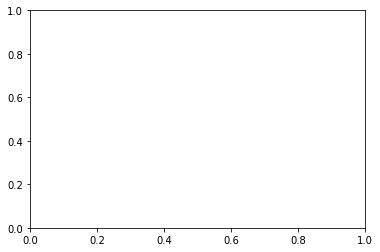
\includegraphics[width=.9\linewidth]{./.ob-jupyter/61d2780d035746e2a1d41c3696837d1141c39f65.png}
\end{center}


\begin{minted}[frame=lines,fontsize=\scriptsize,linenos]{python}
import matplotlib.pyplot as plt
import numpy.random as rnd
from matplotlib.patches import Ellipse

NUM = 250

ells = [Ellipse(xy=rnd.rand(2)*10, width=rnd.rand(), height=rnd.rand(), angle=rnd.rand()*360)
        for i in range(NUM)]

fig = plt.figure(0)
ax = fig.add_subplot(111, aspect='equal')
for e in ells:
    ax.add_artist(e)
    e.set_clip_box(ax.bbox)
    e.set_alpha(rnd.rand())
    e.set_facecolor(rnd.rand(3))

ax.set_xlim(0, 10)
ax.set_ylim(0, 10)

plt.show()

\end{minted}

\begin{center}
\includegraphics[width=.9\linewidth]{./.ob-jupyter/76e22ac73fecc3e100c2fec5dc003b4e9174a123.png}
\end{center}


\begin{minted}[frame=lines,fontsize=\scriptsize,linenos]{python}
import matplotlib.pyplot as plt
import numpy as np

x = np.arange(6)
y = np.arange(5)
z = x * y[:, np.newaxis]

for i in range(5):
    if i == 0:
        p = plt.imshow(z)
        fig = plt.gcf()
        plt.clim()   # clamp the color limits
        plt.title("Boring slide show")
    else:
        z = z + 2
        p.set_data(z)

    print("step", i)
    plt.pause(0.5)
\end{minted}

step 0
\begin{center}
\includegraphics[width=.9\linewidth]{./.ob-jupyter/aef1c63053ea322cb58f7bbc29a6e45303bb7096.png}
\end{center}
step 1
step 2
step 3
step 4


\begin{minted}[frame=lines,fontsize=\scriptsize,linenos]{python}
import matplotlib.pyplot as plt
import numpy as np
from matplotlib.patches import Ellipse

delta = 45.0  # degrees

angles = np.arange(0, 360 + delta, delta)
ells = [Ellipse((1, 1), 4, 2, a) for a in angles]

a = plt.subplot(111, aspect='equal')

for e in ells:
    e.set_clip_box(a.bbox)
    e.set_alpha(0.1)
    a.add_artist(e)

plt.xlim(-2, 4)
plt.ylim(-1, 3)

plt.show()
\end{minted}

<ipython-input-4-de3ee4e9bc8b>:8: MatplotlibDeprecationWarning: Passing the angle parameter of \_\_init\_\_() positionally is deprecated since Matplotlib 3.6; the parameter will become keyword-only two minor releases later.
  ells = [Ellipse((1, 1), 4, 2, a) for a in angles]
\begin{center}
\includegraphics[width=.9\linewidth]{./.ob-jupyter/fa46ea90207cb60496d5f2e70e5014a9510197d1.png}
\end{center}
\end{document}
